\documentclass[../psets.tex]{subfiles}

\pagestyle{main}
\renewcommand{\leftmark}{Problem Set \thesection}
\setcounter{section}{3}

\begin{document}




\section{Isotope Effects and Kinetics}
\marginnote{11/26:}The questions pertain to the material covered from Thermodynamic Isotope Effects (Nov 5) to Kinetic Rate Laws (Nov 14).
\begin{enumerate}
    \item The following schematic illustrates the six possible kinetic scenarios for the reaction
    \begin{equation*}
        \ce{\textbf{A} <=>[$k_1$][$k_{-1}$] \textbf{B} ->[$k_2$] \textbf{C}}
    \end{equation*}
    of \textbf{A} to \textbf{C} via \textbf{B}.
    \begin{center}
        \includegraphics[width=0.7\linewidth]{PSet4F1.png}
    \end{center}
    \begin{enumerate}
        \item In which of these scenarios would the steady-state approximation \emph{not} be valid? Provide a brief explanation for your answers.
        \begin{proof}
            % For the steady-state approximation to be valid, we need $\cnc{I}\ll\cnc{A}$. This often occurs when $k_{-1}\gg k_1$, and hence we have an endothermic initial equilibrium.  
            The steady-state approximation would not be valid in \fbox{Scenarios \textbf{i}, \textbf{iii}, and \textbf{vi}.}\par
            % Equivalently, we need $k_{-1}\gg k_1$. Both of these conditions define an \emph{endothermic} initial equilibrium
            \underline{\textbf{i}}: The initial equilbrium between \textbf{A} and \textbf{B} is exergonic, and there is a significant barrier before conversion to \textbf{C}. Symbolically, $k_1\gg k_{-1}\gg k_2$. Thus, most of the substrate will exist as \textbf{B}. Since $\cnc{\textbf{B}}\gg\cnc{\textbf{A}}$, the steady-state approximation does not hold.\par
            \underline{\textbf{iii}}: Again, it is easier for \textbf{A} to become \textbf{B} than for \textbf{B} to become \textbf{C}, so most of the substrate will sit as the intermediate.\par
            \underline{\textbf{vi}}: There will be more \textbf{A} than \textbf{B}, but \textbf{B} will accumulate before it converts to \textbf{C}
        \end{proof}
        \item In which of these scenarios would the quasi-equilibrium assumption \emph{not} be valid? Provide a brief explanation for your answers.
        \begin{proof}
            The quasi-equilibrium assumption would not be valid in \fbox{Scenarios \textbf{iv} and \textbf{v}.} In both of these, $k_2\gg k_1$, so it will be hard for \textbf{A} and \textbf{B} to effectively equilibrate before some \textbf{B} starts getting converted to product.
        \end{proof}
        \item Consider a situation where \textbf{A} is isotopically labeled. If isotopic substitution affects only the rate of conversion of \textbf{B} to \textbf{C} (and not from \textbf{A} to \textbf{B}), in which scenarios might you expect to observe an independent rate kinetic isotope effect (KIE)? Please explain.
        \begin{proof}
            Under these assumptions, a KIE would be observed when the second step is rate-determining. Recall that the rate-determining step is the step that has the largest energy difference relative either to the starting material or to any previous, lower energy intermediate on the diagram. Thus, we might expect to observe a KIE in \fbox{Scenarios \textbf{i}, \textbf{ii}, \textbf{iii}, and \textbf{vi}.}
        \end{proof}
        \item In which scenarios might you expect to observe an independent rate KIE if isotopic substitution affects only the step involving formation of \textbf{B} from \textbf{A} (and not from \textbf{B} to \textbf{C})?
        \begin{proof}
            When the first step is rate-determining, we'll definitely see a KIE. But even when it is not, KIEs will affect $\cnc{\textbf{B}}$, altering the rate of the RDS! Thus, \fbox{all scenarios} display KIEs.
        \end{proof}
    \end{enumerate}
    \pagebreak
    \item Consider the following reaction.
    \begin{center}
        \footnotesize
        \schemestart
            \chemfig{*6(-(-OMe)=-=(-(-[4]Me)(-[2]Me)-[0]\charge{135=$\oplus$}{N}(-[0])(-[:-60])-[:60]\charge{45=$\ominus$}{O})-=)}
            \arrow{->[$\Delta$]}
            \chemfig{*6(-(-OMe)=-=(-(-[:150]Me)=[:30])-=)}
            \arrow{0}[,0.1]\+{,,-2.2em}
            \chemfig{Me-[:-30]N(-[6]Me)-[:30]OH}
        \schemestop
    \end{center}
    \begin{enumerate}
        \item The mechanism for this reaction could proceed via a concerted pathway or a stepwise pathway. Provide arrow-pushing mechanisms for both processes.
        \begin{proof}
            \underline{Concerted}: This is an E\textsubscript{i} mechanism!
            \begin{center}
                \vspace{1em}
                \footnotesize
                \schemestart
                    \chemfig{*6(-(-OMe)=-=(-(-[:-171]Me)*5([:54,1.3]-[@{3}]@{N}\charge{[extra sep=4pt]30=$\oplus$}{N}(-[:-74,1])(-[:-34,1])-@{O}\charge{45=$\ominus$}{O}-[,,,,opacity=0]@{H}H-[@{1}]H_2C-[@{2}]))-=)}
                    \arrow
                    \chemfig{*6(-(-OMe)=-=(-(-[:150]Me)=[:30])-=)}
                    \arrow{0}[,0.1]\+{,,-2.2em}
                    \chemfig{Me-[:-30]N(-[6]Me)-[:30]OH}
                \schemestop
                \chemmove{
                    \draw [curved arrow={9pt}{2pt}] (O) to[out=45,in=45,out looseness=2.5,in looseness=2] (H);
                    \draw [curved arrow={2pt}{2pt}] (1) to[bend left=54] (2);
                    \draw [curved arrow={2pt}{2pt}] (3) to[bend left=80,looseness=2] (N);
                }
            \end{center}
            \underline{Stepwise}: This is an E\textsubscript{1}-type mechanism!
            \begin{center}
                \vspace{1em}
                \footnotesize
                \schemestart
                    \chemfig{*6(-(-OMe)=-=(-(-[4]Me)(-[2]Me)-[@{3}0]@{N}\charge{-135=$\oplus$}{N}(-[0])(-[:-60])-[:60]\charge{45=$\ominus$}{O})-=)}
                    \arrow
                    \chemfig{*6(-(-OMe)=-=(-\charge{[extra sep=5pt]90=$\oplus$}{}(-[:150]Me)-[@{2}:30]-[@{1}:-30]@{H}H)-=)}
                    \arrow{0}[,0.1]\+{,,-2.2em}
                    \chemfig{Me-[:-30]N(-[6]Me)-[:30]@{O}\charge{45=$\ominus$}{O}}
                    \arrow
                    \chemfig{*6(-(-OMe)=-=(-(-[:150]Me)=[:30])-=)}
                    \arrow{0}[,0.1]\+{,,-2.2em}
                    \chemfig{Me-[:-30]N(-[6]Me)-[:30]OH}
                \schemestop
                \chemmove{
                    \draw [curved arrow={2pt}{2pt}] (3) to[bend left=80,looseness=2] (N);
                    % 
                    \draw [curved arrow={9pt}{2pt}] (O) to[out=45,in=45,out looseness=1.5] (H);
                    \draw [curved arrow={2pt}{2pt}] (1) to[bend left=60] (2);
                }
            \end{center}
        \end{proof}
        \item When the two benzylic methyl groups were deuterated, kinetic isotope effects (KIEs) of 5 and 1.2 were measured in toluene and DMF respectively. Suggest a possible explanation for the observed KIEs.
        \begin{proof}
            A large, likely primary KIE of 5 suggests that \ce{C-H/D} bond cleavage is part of the RDS. Since the RDS of the concerted mechanism (the only step) involves \ce{C-H/D} bond cleavage and the RDS of the stepwise mechanism (likely the first step, as is typical of E\textsubscript{1}-type mechanisms) does not involve \ce{C-H/D} bond cleavage, the concerted mechanism is likely active in toluene.\par
            A small, likely secondary KIE of 1.2 suggests that \ce{C-H/D} bond cleavage is \emph{not} part of the RDS. Thus, for analogous reasons to the above, the stepwise E\textsubscript{1}-type mechanism is likely active in DMF.
        \end{proof}
        \pagebreak
        \item When the reaction was run at two different temperatures and in two different solvents, the following rate data were obtained. Compare the activation enthalpy ($\Delta H^\ddagger$) and activation entropy ($\Delta S^\ddagger$) of the reactions in toluene and in DMF. Suggest a possible explanation for the observed differences.
        \begin{center}
            \includegraphics[width=0.4\linewidth]{PSet4F2.png}
        \end{center}
        \begin{proof}
            Although it is not possible to obtain absolute values (e.g., in \si{\kilo\calorie\per\mole}) for $\Delta H^\ddagger$ and $\Delta S^\ddagger$ from this data, a modified Eyring plot can compare the magnitudes of these quantities between the two reactions. For toluene, the line through
            \begin{align*}
                \left( \frac{1}{273+60},\ln(1) \right)&&
                \left( \frac{1}{273+110},\ln(50) \right)
            \end{align*}
            has slope $m=-9979$ and $y$-intercept $b=29.97$, so $\Delta H^\ddagger_\text{rel}=19.74$ and $\Delta S^\ddagger_\text{rel}=0.0593$. For DMF, the line through
            \begin{align*}
                \left( \frac{1}{273+60},\ln(10) \right)&&
                \left( \frac{1}{273+110},\ln(\num{500000}) \right)
            \end{align*}
            has slope $m=-27600$ and $y$-intercept $b=85.18$, so $\Delta H^\ddagger_\text{rel}=54.6$ and $\Delta S^\ddagger_\text{rel}=0.169$.\par
            It follows that the reaction in DMF --- which proceeds via the stepwise mechanism, per part (b) --- has both a higher enthalpy and entropy of activation. It makes sense that it should have a higher enthalpy of activation since the RDS involves the formation of a high-energy carbocation intermediate. It also makes sense that it should have a higher entropy of activation because the introduction of charged species into a polar aprotic solvent will disrupt the random bonding of the solvent to itself and introduce highly ordered ion cages.
        \end{proof}
    \end{enumerate}
    \pagebreak
    \item In nonpolar solvents, compound \textbf{1} reacts thermally with \textbf{2} to give only \emph{endo} \textbf{3}.
    \begin{center}
        \includegraphics[width=0.55\linewidth]{PSet4F3.png}
    \end{center}
    Using small amounts of \textbf{1} and `flooding' with \textbf{2}, it has been established that the rate is pseudo-first-order in $\cnc{\textbf{1}}$. Measuring the pseudo-first-order rate constant $\kobs$ at several different concentrations of excess \textbf{2} gives a plot of the type shown below.
    \begin{center}
        \includegraphics[width=0.35\linewidth]{PSet4F4.png}
    \end{center}
    Compound \textbf{1}, deuterated at phosphorus, undergoes exchange of \ce{D} with both $\alpha$-hydrogens, as shown below. At low concentrations of \textbf{2}, the \ce{H}/\ce{D} exchange rate is rapid compared to the rate of formation of \textbf{3}. At `saturating' concentrations of \textbf{2}, the formation of \textbf{3} occurs faster than \ce{H}/\ce{D} exchange.
    \begin{center}
        \includegraphics[width=0.7\linewidth]{PSet4F5.png}
    \end{center}
    \begin{enumerate}
        \item Write a full mechanism and a rate law for the formation of \textbf{3} that is consistent with these observations.
        \begin{proof}
            A full mechanism consistent with these observations is
            \begin{center}
                \includegraphics[width=0.8\linewidth]{PSet4Q3a.png}
            \end{center}
            A rate law consistent with these observations is
            \begin{equation*}
                \boxed{\rate = \frac{k_1k_2\cnc{\textbf{1}}\cnc{\textbf{2}}}{k_{-1}+k_2\cnc{\textbf{2}}}}
            \end{equation*}
        \end{proof}
        \pagebreak
        \item Explain how your mechanism accounts for the labeling and kinetic behavior.
        \begin{proof}
            % Nonpolar solvents: ??
            % Exclusive formation of \emph{endo}: Diels-Alder with EWG/diene pairing.
            % Rapid suprafacial $[1,5]$-sigmatropic \ce{H}-atom shifts.
            % Saturating conditions give faster formation of \textbf{3} than sigmatropic: Peak in energy diagram for $k_2$ must be lower than the peak for $k_{-1}$.
            % QEA vs. SSA regime: Derive a rate law for each, and then use the middle graph to confirm that it's SSA. Thus, $\textbf{1*}+\textbf{2}$ is higher in energy than $\textbf{1}+\textbf{2}$.
            % That the reaction proceeds, plus formating of \ce{C-C} $\sigma$-bonds being a big driving force: Reaction is exergonic overall.

            We begin by developing a plausible arrow-pushing mechanism for the overall indicated transformation. Nonpolar solvents, thermal reactivity, a starting material (\textbf{2}) with two strong EWGs, and \emph{endo}-selectivity suggests that \textbf{3} was ultimately formed by a $[4+2]$ cycloaddition. Taking the six-membered ring in \textbf{3} to be a full retron for a $[4+2]$ cycloaddition, we can predict \textbf{1*} and \textbf{2} as starting materials. Indeed, \textbf{1*} and \textbf{2} would react in the forward direction via the indicated transition state, with bonds being formed between the HOMO of \textbf{1*} and the full LUMO of \textbf{2}; \emph{endo}-selectivity is secured by the two secondary orbital interactions indicated with dashed lines. This just leaves the question of where \textbf{1*} could have come from. One possible option is from \textbf{1} via a suprafacial $[1,5]$-sigmatropic \ce{H}-atom shift. Such pathways are very common for such doubly unsaturated systems, so this is a reasonable hypothesis.\par
            Let's now see why this plausible mechanism is defensible based on the given data, and in the process derive the above rate law. To begin, a simplified chemical equation is
            \begin{equation*}
                \ce{\textbf{1} <=>[$k_1$][$k_{-1}$] \textbf{1*} ->[\textbf{2}][$k_2$] \textbf{3}}
            \end{equation*}
            Based on this equation, we would predict that
            \begin{equation*}
                \rate = \dv{\cnc{\textbf{3}}}{t} = k_2\cnc{\textbf{1*}}\cnc{\textbf{2}}
            \end{equation*}
            To (analytically) express $\cnc{\textbf{1*}}$ in terms of $\cnc{\textbf{1}}$, we may choose between four possible simplifying assumptions:
            \begin{itemize}
                \item The steady-state approximation.
                \item The steady-state approximation, accounting for $\cnc[T]{\textbf{1}}$.
                \item The quasi-equilibrium assumption.
                \item The quasi-equilibrium assumption, accounting for $\cnc[T]{\textbf{1}}$.
            \end{itemize}
            Using these assumptions, we may derive the following four rate laws, respectively.
            \begin{align*}
                \rate &= \frac{k_1k_2\cnc{\textbf{1}}\cnc{\textbf{2}}}{k_{-1}+k_2\cnc{\textbf{2}}}&
                \rate &= \frac{k_1k_2\cnc[T]{\textbf{1}}\cnc{\textbf{2}}}{k_1+k_{-1}+k_2\cnc{\textbf{2}}}&
                \rate &= \frac{k_1k_2}{k_{-1}}\cnc{\textbf{1}}\cnc{\textbf{2}}&
                \rate &= \frac{k_1k_2}{k_1+k_{-1}}\cnc{\textbf{1}}\cnc{\textbf{2}}
            \end{align*}
            Both equations derived under the quasi-equilibrium assumption fail to account for the saturation kinetics on display in the $\kobs$ vs. $\cnc{\textbf{2}}$ plot, so we can rule them out. Thus, this reaction must occur in a regime subject to the steady-state approximation. It follows that $k_{-1}\gg k_1$, so we may additionally neglect the $k_1$ term in the denominator of the fourth option, leaving the indicated rate law as our choice.\par
            Additionally, observe that in the limiting case of `flooding' with \textbf{2}, $k_2\cnc{\textbf{2}}\gg k_{-1}$. This allows the rate law to collapse to
            \begin{equation*}
                \rate = k_1\cnc{\textbf{1}}
                = \kobs\cnc{\textbf{1}}
            \end{equation*}
            corresponding to the observation of that the reaction is pseudo-first-order in \textbf{1} under these conditions!\par
            Furthermore, the proposed reversible first step would account for the hydrogen-deuterium exchange at the symmetric $\alpha$-carbons (even in the absence of \textbf{2}): \ce{D} could migrate from the phosphorus center to either $\alpha$-carbon, and then either \ce{D} or \ce{H} could migrate back.\par
            The final observation regarding the relative rates of \ce{H}/\ce{D} exchange vs. the rate of formation of \textbf{3} will be useful in part (c).
        \end{proof}
        \pagebreak
        \item Draw reaction coordinate energy diagrams at the limiting cases where $\cnc{\textbf{2}}$ is\dots
        \begin{enumerate}[label={\roman*)}]
            \item Very low;
            \begin{proof}
                {\color{white}hi}
                \begin{center}
                    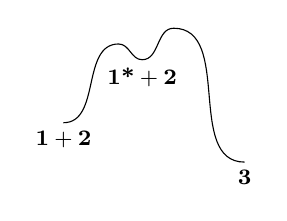
\begin{tikzpicture}
                        \footnotesize
                        \draw (0,0) node[below]{$\textbf{1}+\textbf{2}$}
                            to[out=0,in=180] (0.7,1)
                            to[out=0,in=180] (1,0.8) node[below]{$\textbf{1*}+\textbf{2}$}
                            to[out=0,in=180] (1.4,1.2)
                            to[out=0,in=180] (2.3,-0.5) node[below]{$\textbf{3}$}
                        ;
                    \end{tikzpicture}
                \end{center}
                Since this reaction obeys the steady-state approximation as discussed in part (b), not much \textbf{1*} is ever formed. Thus, $\textbf{1*}+\textbf{2}$ should always be higher in energy than $\textbf{1}+\textbf{2}$. Additionally, since the reaction proceeds, it should always be exergonic. Finally, the difference in the heights of the transition states comes from the data that \ce{H}/\ce{D} exchange is faster than formation of \textbf{3} at low concentrations of \textbf{2}; this observation implies a lower barrier for $\textbf{1*}+\textbf{2}$ to return to the reactants than proceed on to the products.
            \end{proof}
            \item Very high.
            \begin{proof}
                {\color{white}hi}
                \begin{center}
                    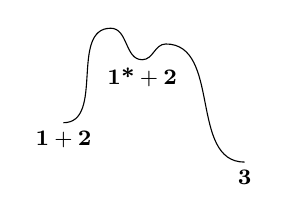
\begin{tikzpicture}
                        \footnotesize
                        \draw (0,0) node[below]{$\textbf{1}+\textbf{2}$}
                            to[out=0,in=180] (0.6,1.2)
                            to[out=0,in=180] (1,0.8) node[below]{$\textbf{1*}+\textbf{2}$}
                            to[out=0,in=180] (1.3,1)
                            to[out=0,in=180] (2.3,-0.5) node[below]{$\textbf{3}$}
                        ;
                    \end{tikzpicture}
                \end{center}
                The analysis is identical to the part (c.i), except that conversion to the products now occurs faster, so its barrier should be lower.
            \end{proof}
        \end{enumerate}
    \end{enumerate}
    \pagebreak
    \item 
    \begin{enumerate}
        \item Estimate the magnitudes of the equilibrium constants ($K_1$, $K_2$) for the following reactions. Provide explanations.
        \begin{center}
            \includegraphics[width=0.5\linewidth]{PSet4F6.png}
        \end{center}
        \begin{proof}
            \ce{C-D} bonds have a slightly greater BDE than \ce{C-H} bonds. Thus, they hold onto their electrons more tightly and are less likely to participate in stabilizing interactions like hyperconjugation. Essentially, carbocations subject to $\sigma_{\ce{CH}}\to p_{\ce{C}}$ hyperconjugation will be more stable than those subject to $\sigma_{\ce{CD}}\to p_{\ce{C}}$ hyperconjugation, all else being equal. Thus, we should have
            \begin{equation*}
                \boxed{K_1 > 1}
            \end{equation*}
            Note that $K_1$ will likely be only slightly greater than one: When we compared diaxial interactions between methyl groups and perdeuterated methyl groups in class, $\Keq$ was $1.042$.\par
            For $K_2$, the $\sigma_{\ce{CD}}$-orbital is orthogonal to the carbocation's $p_{\ce{C}}$ orbital, so it cannot stabilize it anyway. Thus, we should have
            \begin{equation*}
                \boxed{K_2 \approx 1}
            \end{equation*}
        \end{proof}
        \item Estimate the magnitudes of $\text{KIE}_1$ and $\text{KIE}_2$ for the following solvolysis reactions. Provide explanations.
        \begin{center}
            \includegraphics[width=0.55\linewidth]{PSet4F7.png}
        \end{center}
        \begin{proof}
            The same effects at play in part (a) are also in effect here, except that the type of hyperconjugation is now anomeric $\sigma_{\ce{C-H/D}}\to\sigma^*_{\ce{C-O}}$ donation. A lack of orbital alignment for the top reaction means that
            \begin{equation*}
                \boxed{\text{KIE}_1 \approx 1}
            \end{equation*}
            Orbital alignment in the bottom case will predict a small normal secondary KIE:
            \begin{equation*}
                \boxed{\text{KIE}_2 \in (1,1.5)}
            \end{equation*}
        \end{proof}
    \end{enumerate}
\end{enumerate}




\end{document}